%% =======================================================
%% Actividad 7: Simulación y análisis de variables aleatorias
%%
%% Compilar desde actividades/: ./compilar.sh act07
%% Las figuras de img/ se generan con: python act07.py
%% =======================================================

%% ---- CONFIGURACIÓN ------------------------

\documentclass[11pt,letterpaper]{article}

\usepackage[indice]{tecnm}
\usepackage[T1]{fontenc}
\usepackage{amsmath}
\usepackage{xcolor}
\usepackage[most]{tcolorbox} % Carga tcolorbox con soporte para listings y saltos de página
\tcbuselibrary{listings, skins, breakable}
\setlength{\emergencystretch}{3em} % Evita líneas desbordadas por palabras en \texttt

% Paleta de colores (estilo GitHub Light / VS Code)
\definecolor{codebg}{HTML}{F8F9FA}       % Fondo del código
\definecolor{codehead}{HTML}{E9ECEF}     % Fondo de la barra de título
\definecolor{codeborder}{HTML}{CED4DA}   % Borde de la tarjeta
\definecolor{codetitle}{HTML}{212529}    % Texto del título
\definecolor{codekw}{HTML}{0550AE}       % Palabras clave (import, def, for...)
\definecolor{codefunc}{HTML}{8250DF}     % Funciones y métodos (describe, groupby...)
\definecolor{codestr}{HTML}{0A3069}      % Strings
\definecolor{codecomm}{HTML}{6E7781}     % Comentarios
\definecolor{codenum}{HTML}{8C959F}      % Números de línea
\definecolor{codeid}{HTML}{24292F}       % Texto general

% Configuración base de listings
\lstdefinestyle{pythonestilo}{
  language=Python,
  basicstyle=\ttfamily\footnotesize\color{codeid},
  keywordstyle=\color{codekw}\bfseries,
  keywordstyle=[2]\color{codefunc}, % Estilo secundario para métodos de datos
  stringstyle=\color{teal!80!black},
  commentstyle=\color{codecomm}\itshape,
  morekeywords={as, True, False, None, with, yield, lambda},
  morekeywords=[2]{print, len, sum, max, DataFrame, Series, value_counts, reindex, mean, std, var, randint, normal, seed, cumsum, chisquare, pdf, cdf, hist, bar, plot, axhline, axvline, fill_between, subplots, figure, concat, nunique, load_iris, diff, sort, unique},
  numbers=left,
  numberstyle=\tiny\ttfamily\color{codenum},
  stepnumber=1,
  numbersep=10pt,
  showstringspaces=false,
  morestring=[b]{"""},
  tabsize=4,
  breaklines=true,
  breakatwhitespace=true,
  columns=flexible,
  keepspaces=true,
  literate=
    {á}{{\'a}}1 {é}{{\'e}}1 {í}{{\'i}}1 {ó}{{\'o}}1 {ú}{{\'u}}1
    {Á}{{\'A}}1 {É}{{\'E}}1 {Í}{{\'I}}1 {Ó}{{\'O}}1 {Ú}{{\'U}}1
    {ñ}{{\~n}}1 {Ñ}{{\~N}}1 {¿}{{?`}}1 {¡}{{!`}}1 {°}{{$^\circ$}}1
}

% Definición del entorno personalizado \begin{codigo}{Título}{etiqueta}
% \newtcblisting[auto counter, number within=section]{codigo}[2][]{
\newtcblisting[auto counter]{codigo}[2][]{
  listing only,
  breakable,                    % Permite que el bloque se divida si pasa de página
  enhanced,
  colback=codebg,
  colframe=codeborder,
  colbacktitle=codehead,
  coltitle=codetitle,
  fonttitle=\bfseries\small\sffamily,
  boxrule=0.6pt,
  arc=4pt,                      % Bordes redondeados
  left=20pt,                    % Espacio izquierdo para los números de línea
  right=8pt,
  top=6pt,
  bottom=6pt,
  toptitle=4pt,
  bottomtitle=4pt,
  before skip=12pt,
  after skip=12pt,
  listing options={style=pythonestilo},
  title={Código \thetcbcounter: #2},
  #1
}

% Paleta para salida de consola (estilo terminal limpia)
\definecolor{termbg}{HTML}{212529}      % Fondo oscuro tipo terminal
\definecolor{termhead}{HTML}{343A40}    % Barra superior
\definecolor{termtext}{HTML}{F8F9FA}    % Texto claro de alta legibilidad
\definecolor{termborder}{HTML}{495057}  % Borde

% Entorno \begin{consola}[label=out:iris]{Título}
\newtcblisting[auto counter]{consola}[2][]{
  listing only,
  breakable,
  colback=termbg,
  colframe=termborder,
  colbacktitle=termhead,
  coltitle=termtext,
  colupper=termtext,
  fonttitle=\bfseries\small\sffamily,
  boxrule=0.6pt,
  arc=4pt,
  left=8pt,
  right=8pt,
  top=6pt,
  bottom=6pt,
  toptitle=4pt,
  bottomtitle=4pt,
  before skip=12pt,
  after skip=12pt,
  listing options={
    basicstyle=\ttfamily\scriptsize\color{termtext}, % \scriptsize evita que las tablas de Pandas se partan de línea
    breaklines=true,
    columns=fixed,        % Mantiene alineadas las columnas de Pandas
    keepspaces=true,
    showstringspaces=false,
    literate=
      {á}{{\'a}}1 {é}{{\'e}}1 {í}{{\'i}}1 {ó}{{\'o}}1 {ú}{{\'u}}1
      {Á}{{\'A}}1 {É}{{\'E}}1 {Í}{{\'I}}1 {Ó}{{\'O}}1 {Ú}{{\'U}}1
      {ñ}{{\~n}}1 {Ñ}{{\~N}}1 {°}{{$^\circ$}}1
  },
  title={Salida \thetcbcounter: #2},
  #1
}

%% ---- DATOS DE LA MATERIA ------------------------

\materia{Modelos Estadísticos para el Aprendizaje \\ Automático y Ciencia de Datos}
\actividad{Tema 2.1
Variables Aleatorias: Tipos, Ejemplos, Representación Computacional \\ Actividad 7 - Simulación y Análisis de Variables Aleatorias}

\profesor{Dr. José Ismael Ojeda Campaña}
%\fecha{15 de octubre de 2026}    % opcional; por defecto es la fecha de hoy

\begin{document}
\portada
\indicegeneral

%% ---- CONTENIDO ---------------------------------

\section{Introducción}

Los fenómenos del mundo real rara vez son deterministas: el resultado de lanzar un dado, la altura de una persona o la temperatura de un día no pueden conocerse con exactitud antes de observarlos. Las variables aleatorias son la herramienta matemática que permite describir esta incertidumbre mediante una distribución de probabilidad, y son la base de los modelos predictivos del aprendizaje automático \parencite{tecnm2026_documento_fuente,brownlee2020}.

En este documento se estudia la diferencia entre los dos tipos principales de variables aleatorias, las discretas y las continuas, mediante simulación en Python. Primero se simulan 1000 lanzamientos de un dado balanceado, un ejemplo clásico de variable discreta, y se comparan sus frecuencias relativas con la probabilidad teórica de $1/6$. Después se simulan 500 valores de una distribución normal con media 100 y desviación estándar 15, un ejemplo de variable continua, y se comparan la media y la desviación estándar de la muestra con los parámetros de la población. Finalmente, se comparan ambos tipos de variables y se identifican ejemplos de cada uno en los conjuntos de datos Weather e Iris.

\section{Marco conceptual}

\subsection{Variables aleatorias}

Una variable aleatoria es una cantidad de interés cuyo valor verdadero es desconocido. Para obtener información sobre ella se diseñan y realizan experimentos, pero ninguna medición permite conocerla con exactitud. En su lugar, la variable se describe mediante una distribución de probabilidad, que determina la probabilidad de que ocurra cada uno de sus valores \parencite{tecnm2026_documento_fuente,bonamente2017}. Al repetir la medición aumenta el conocimiento sobre esa distribución, por lo que conviene realizar tantas mediciones como sea posible: las mediciones agrupadas forman la distribución muestral, que se aproxima a la distribución teórica a medida que crece el número de observaciones \parencite{bonamente2017}.

Hay dos clases principales de variables aleatorias \parencite{tecnm2026_documento_fuente,brownlee2020}:

\begin{itemize}
    \item \textbf{Discreta:} sus valores se toman de un conjunto finito (o numerable) de estados, por ejemplo, los colores de un automóvil o las caras de un dado.
    \item \textbf{Continua:} sus valores se extraen de un rango de números reales, por ejemplo, la altura de las personas.
\end{itemize}

\subsection{Distribuciones de probabilidad}

Una distribución de probabilidad es un resumen de las probabilidades para los valores de una variable aleatoria \parencite{tecnm2026_documento_fuente}. Su forma de describirla depende del tipo de variable.

\paragraph{Variables discretas.} La distribución se describe con una función de masa de probabilidad, $p(x) = P(X = x)$, que asigna una probabilidad a cada valor posible y cuyas probabilidades suman 1 \parencite{brownlee2020}. En un dado balanceado, las seis caras son igualmente probables, por lo que la variable sigue una distribución uniforme discreta:
\begin{equation}
    P(X = k) = \frac{1}{6}, \qquad k = 1, 2, \ldots, 6.
\end{equation}
Su valor esperado y su varianza son
\begin{equation}
    E[X] = \sum_{k=1}^{6} k \cdot \frac{1}{6} = 3.5, \qquad
    \operatorname{Var}[X] = \sum_{k=1}^{6} (k - 3.5)^2 \cdot \frac{1}{6} = \frac{35}{12} \approx 2.917.
\end{equation}

\paragraph{Variables continuas.} Como una variable continua puede tomar infinitos valores, la probabilidad de un valor exacto es cero. La distribución se describe con una función de densidad $f(x)$, y las probabilidades se calculan como áreas bajo esa curva, $P(a < X \leq b) = \int_a^b f(x)\,dx$ \parencite{tecnm2026_documento_fuente,brownlee2020}. La distribución continua más importante es la normal o gaussiana, con media $\mu$ y desviación estándar $\sigma$ \parencite{tecnm2026_documento_fuente}:
\begin{equation}
    f(x) = \frac{1}{\sigma \sqrt{2\pi}} \exp\!\left( -\frac{(x - \mu)^2}{2\sigma^2} \right).
\end{equation}
Es simétrica respecto a $\mu$ y concentra cerca del 68\,\%, 95\,\% y 99.7\,\% de los valores a una, dos y tres desviaciones estándar de la media \parencite{bonamente2017}.

\subsection{Parámetros poblacionales y estadísticos muestrales}

Los parámetros de una distribución, como $\mu$ y $\sigma$, describen a la población completa. A partir de una muestra de $n$ observaciones se calculan estadísticos que los estiman: la media muestral $\bar{x}$ y la desviación estándar muestral $s$ \parencite{bonamente2017}. Estos estimadores no coinciden exactamente con los parámetros, porque cada muestra es distinta. La precisión de la media muestral se mide con su error estándar,
\begin{equation}
    \text{EE}(\bar{x}) = \frac{\sigma}{\sqrt{n}},
\end{equation}
que disminuye al aumentar el tamaño de la muestra \parencite{bruce2020}. Del mismo modo, la frecuencia relativa con que aparece un valor discreto se acerca a su probabilidad teórica cuando el número de repeticiones del experimento crece \parencite{bonamente2017}.

\subsection{Rol en los modelos de inteligencia artificial}

El aprendizaje automático desarrolla modelos predictivos a partir de datos inciertos. La incertidumbre surge por el ruido en las observaciones, por la cobertura incompleta del dominio y por la imperfección de los propios modelos \parencite{tecnm2026_documento_fuente,brownlee2020}. Las variables aleatorias permiten cuantificar esta incertidumbre. Por ejemplo, la salida de un clasificador puede modelarse como una variable aleatoria discreta sobre las clases posibles, y modelos como Naive Bayes estiman la probabilidad de cada clase usando distribuciones discretas para las características categóricas y distribuciones continuas, como la normal, para las numéricas \parencite{tecnm2026_documento_fuente}. Por eso, identificar correctamente el tipo de cada variable es un paso previo a elegir el modelo adecuado.

\section{Descripción de la actividad}

\textbf{Objetivo:} Comprender la diferencia entre variables aleatorias discretas y continuas mediante la simulación y visualización de sus distribuciones \parencite{tecnm2026_documento_fuente}.

La actividad consta de tres tareas:

\begin{description}
    \item[a) Simulación de variables discretas.] Generar 1000 lanzamientos de un dado balanceado con \texttt{numpy.random.randint}, calcular la frecuencia relativa de cada cara, compararla con la probabilidad teórica ($1/6$) y graficar los resultados en un diagrama de barras.
    \item[b) Simulación de variables continuas.] Generar 500 muestras de una distribución normal con media 100 y desviación estándar 15, representarlas en un histograma superpuesto con la curva de densidad teórica, y calcular la media y la desviación estándar muestrales para compararlas con los parámetros poblacionales.
    \item[c) Análisis comparativo.] Elaborar una tabla comparativa entre variables discretas y continuas, e identificar ejemplos reales de cada tipo en conjuntos de datos como el Weather Dataset o el Iris Dataset.
\end{description}

\section{Desarrollo}

Las tres tareas se resolvieron en el script \texttt{act07.py}, que usa \texttt{numpy}, \texttt{pandas}, \texttt{scipy}, \texttt{matplotlib} y \texttt{scikit-learn}. Las simulaciones usan la semilla 7 para que los resultados sean reproducibles, y las figuras se guardan como imágenes PNG en la carpeta \texttt{img/}. El Código~\ref{cod:comun} contiene las importaciones y la función auxiliar \texttt{guardar()}, que además muestra las figuras en pantalla cuando el código se ejecuta en un cuaderno. El cuaderno interactivo puede consultarse en Google Colab:

\begin{center}
    \url{https://colab.research.google.com/drive/1kCUnzGrp2TGgZmgZIi1f9zGQ2CGSI-un?usp=sharing}
\end{center}

\begin{codigo}[label=cod:comun]{Importaciones y función auxiliar}
import os

import matplotlib

# En Colab o Jupyter no existe __file__; ahí las figuras también se muestran en pantalla
EN_NOTEBOOK = '__file__' not in globals()
if not EN_NOTEBOOK:
    matplotlib.use('Agg')  # Como script, genera las figuras como archivos PNG sin abrir ventanas

import matplotlib.pyplot as plt
import numpy as np
import pandas as pd
from scipy import stats
from sklearn.datasets import load_iris

pd.set_option('display.width', 100)

# Carpeta donde se guardan las figuras que se incluyen en el reporte
BASE = os.getcwd() if EN_NOTEBOOK else os.path.dirname(os.path.abspath(__file__))
CARPETA_IMG = os.path.join(BASE, 'img')
os.makedirs(CARPETA_IMG, exist_ok=True)


def guardar(nombre):
    """Guarda la figura actual en la carpeta img/ y la muestra si se ejecuta en un notebook."""
    plt.tight_layout()
    plt.savefig(os.path.join(CARPETA_IMG, nombre), dpi=150)
    if EN_NOTEBOOK:
        plt.show()
    plt.close()
\end{codigo}

\subsection{Tarea a: Simulación de una variable discreta}

Los 1000 lanzamientos se generaron con \texttt{np.random.randint(1, 7, 1000)}; el límite superior se excluye, por lo que los valores posibles son del 1 al 6. La función \texttt{tabla\_frecuencias()} cuenta cuántas veces salió cada cara y calcula su frecuencia relativa y su diferencia con la probabilidad teórica. Como extensiones, se calcularon la media y la varianza de los lanzamientos para compararlas con $E[X] = 3.5$ y $\operatorname{Var}[X] = 35/12$, y se aplicó una prueba chi-cuadrada de bondad de ajuste con \texttt{stats.chisquare()}. Esta prueba evalúa si las diferencias entre las frecuencias observadas y las esperadas ($1000/6 \approx 166.7$ por cara) pueden atribuirse al azar; un valor $p > 0.05$ indica que los datos son compatibles con un dado balanceado.

\begin{codigo}[label=cod:a]{Tarea a: 1000 lanzamientos de un dado}
N_LANZAMIENTOS = 1000
CARAS = np.arange(1, 7)
P_TEORICA = 1 / 6

np.random.seed(7)
lanzamientos = np.random.randint(1, 7, N_LANZAMIENTOS)  # el límite superior se excluye


def tabla_frecuencias(datos, valores, p_teorica):
    """Frecuencia absoluta y relativa de cada valor, comparada con la probabilidad teórica."""
    conteos = pd.Series(datos).value_counts().reindex(valores, fill_value=0)
    tabla = pd.DataFrame({'Frecuencia': conteos,
                          'Relativa': conteos / len(datos),
                          'Teórica': p_teorica})
    tabla['Diferencia'] = tabla['Relativa'] - tabla['Teórica']
    tabla.index.name = 'Cara'
    return tabla


tabla_dado = tabla_frecuencias(lanzamientos, CARAS, P_TEORICA)

# Media y varianza teóricas de un dado balanceado: E[X] = 3.5, Var[X] = 35/12
media_teorica = np.sum(CARAS * P_TEORICA)
var_teorica = np.sum((CARAS - media_teorica) ** 2 * P_TEORICA)

# Prueba chi-cuadrada de bondad de ajuste: ¿las frecuencias son compatibles con 1/6?
chi2 = stats.chisquare(tabla_dado['Frecuencia'], f_exp=[N_LANZAMIENTOS * P_TEORICA] * 6)

print("=== a) Variable discreta: 1000 lanzamientos de un dado ===")
print(tabla_dado.round(4))
print(f"\nSuma de frecuencias relativas: {tabla_dado['Relativa'].sum():.4f}")
print(f"Máxima diferencia absoluta con 1/6: {tabla_dado['Diferencia'].abs().max():.4f}")
print(f"Media muestral: {lanzamientos.mean():.4f}   media teórica: {media_teorica:.4f}")
print(f"Varianza muestral: {lanzamientos.var(ddof=1):.4f}   varianza teórica: {var_teorica:.4f}")
print(f"Prueba chi-cuadrada: estadístico = {chi2.statistic:.3f}, p = {chi2.pvalue:.3f}")

# Diagrama de barras de las frecuencias relativas
plt.figure(figsize=(7, 4.5))
barras = plt.bar(CARAS, tabla_dado['Relativa'], color='skyblue', edgecolor='black',
                 label='Frecuencia relativa observada')
plt.axhline(P_TEORICA, color='red', linestyle='--', linewidth=2,
            label=f'Probabilidad teórica (1/6 = {P_TEORICA:.4f})')
for barra, frecuencia in zip(barras, tabla_dado['Frecuencia']):
    plt.text(barra.get_x() + barra.get_width() / 2, barra.get_height() + 0.003,
             str(frecuencia), ha='center', fontsize=9)
plt.title('1000 lanzamientos de un dado balanceado')
plt.xlabel('Cara del dado')
plt.ylabel('Frecuencia relativa')
plt.xticks(CARAS)
plt.ylim(0, 0.22)
plt.legend(loc='lower right')
plt.grid(axis='y', linestyle='--', alpha=0.6)
guardar('a_dado_barras.png')
\end{codigo}

\subsection{Tarea b: Simulación de una variable continua}

Las 500 muestras se generaron con \texttt{np.random.normal(100, 15, 500)}. El histograma se dibujó con \texttt{density=True}, de modo que el área de las barras suma 1 y puede compararse directamente con la densidad teórica, calculada con \texttt{stats.norm.pdf()}. La desviación estándar muestral se calculó con \texttt{ddof=1}, es decir, dividiendo entre $n - 1$. Como extensiones, se calculó el error estándar de la media para juzgar si la diferencia entre $\bar{x}$ y $\mu$ es razonable, y se comparó la proporción de muestras a una, dos y tres desviaciones estándar de la media con la que predice la distribución normal.

\begin{codigo}[label=cod:b]{Tarea b: 500 muestras de una distribución normal}
MU, SIGMA, N_MUESTRAS = 100, 15, 500

np.random.seed(7)
muestras = np.random.normal(MU, SIGMA, N_MUESTRAS)

media_muestral = muestras.mean()
desv_muestral = muestras.std(ddof=1)
error_estandar = SIGMA / np.sqrt(N_MUESTRAS)

comparacion = pd.DataFrame({
    'Poblacional': [MU, SIGMA],
    'Muestral': [media_muestral, desv_muestral],
}, index=['Media', 'Desv. estándar'])
comparacion['Diferencia'] = comparacion['Muestral'] - comparacion['Poblacional']
comparacion['Error relativo (%)'] = comparacion['Diferencia'] / comparacion['Poblacional'] * 100

# Proporción de muestras a 1, 2 y 3 desviaciones estándar de la media poblacional
intervalos = pd.DataFrame({
    'Muestra (%)': [np.mean(np.abs(muestras - MU) <= k * SIGMA) * 100 for k in (1, 2, 3)],
    'Teórica (%)': [(stats.norm.cdf(k) - stats.norm.cdf(-k)) * 100 for k in (1, 2, 3)],
}, index=['[85, 115]', '[70, 130]', '[55, 145]'])

print("\n=== b) Variable continua: 500 muestras de N(100, 15) ===")
print(comparacion.round(3))
print(f"\nError estándar de la media (sigma / raíz de n): {error_estandar:.3f}")
print(f"Diferencia de la media en errores estándar: "
      f"{(media_muestral - MU) / error_estandar:.2f}")
print(f"Mínimo: {muestras.min():.2f}   Máximo: {muestras.max():.2f}")
print("\nProporción de muestras en cada intervalo:")
print(intervalos.round(1))

# Histograma de densidad con la curva teórica superpuesta
plt.figure(figsize=(8, 5))
plt.hist(muestras, bins=25, density=True, color='lightgreen', edgecolor='black',
         label='Histograma de las 500 muestras')
x = np.linspace(MU - 4 * SIGMA, MU + 4 * SIGMA, 300)
plt.plot(x, stats.norm.pdf(x, MU, SIGMA), color='red', linewidth=2,
         label='Densidad teórica N(100, 15)')
plt.axvline(MU, color='red', linestyle='--', linewidth=1, label=f'$\\mu$ = {MU}')
plt.axvline(media_muestral, color='navy', linestyle='-', linewidth=1.5,
            label=f'$\\bar{{x}}$ = {media_muestral:.2f}')
plt.title('Distribución normal: muestra vs. densidad teórica')
plt.xlabel('Valor')
plt.ylabel('Densidad')
plt.legend(fontsize=8)
plt.grid(axis='y', linestyle='--', alpha=0.6)
guardar('b_normal_histograma.png')
\end{codigo}

\subsection{Extensión: convergencia de los estimadores}

Para mostrar cómo la distribución muestral se acerca a la teórica al aumentar las observaciones, se calcularon la frecuencia relativa acumulada de cada cara del dado después de $n = 1, 2, \ldots, 1000$ lanzamientos, y la media acumulada de las muestras normales después de $n = 1, 2, \ldots, 500$ valores. Alrededor de la media acumulada se dibujó la banda $\mu \pm 2\sigma/\sqrt{n}$, dentro de la cual se espera que quede la media muestral en aproximadamente el 95\,\% de los casos.

\begin{codigo}[label=cod:ext]{Extensión: convergencia de los estimadores}
n_valores = np.arange(1, N_LANZAMIENTOS + 1)
# Frecuencia relativa acumulada de cada cara después de n lanzamientos
frecuencia_acumulada = {cara: np.cumsum(lanzamientos == cara) / n_valores for cara in CARAS}
media_acumulada = np.cumsum(muestras) / np.arange(1, N_MUESTRAS + 1)

fig, (ax1, ax2) = plt.subplots(1, 2, figsize=(12, 4.5))
for cara, serie in frecuencia_acumulada.items():
    ax1.plot(n_valores, serie, linewidth=1, label=f'Cara {cara}')
ax1.axhline(P_TEORICA, color='black', linestyle='--', linewidth=1.5, label='1/6')
ax1.set_xscale('log')
ax1.set_ylim(0, 0.5)
ax1.set_title('Dado: frecuencia relativa acumulada')
ax1.set_xlabel('Número de lanzamientos (escala logarítmica)')
ax1.set_ylabel('Frecuencia relativa')
ax1.legend(fontsize=7, ncol=2)
ax1.grid(linestyle='--', alpha=0.5)

n_normal = np.arange(1, N_MUESTRAS + 1)
ax2.plot(n_normal, media_acumulada, color='navy', linewidth=1.2, label='Media muestral acumulada')
ax2.axhline(MU, color='red', linestyle='--', linewidth=1.5, label=f'$\\mu$ = {MU}')
ax2.fill_between(n_normal, MU - 2 * SIGMA / np.sqrt(n_normal), MU + 2 * SIGMA / np.sqrt(n_normal),
                 color='red', alpha=0.12, label='$\\mu \\pm 2\\sigma/\\sqrt{n}$')
ax2.set_xscale('log')
ax2.set_ylim(70, 130)
ax2.set_title('Normal: media muestral acumulada')
ax2.set_xlabel('Número de muestras (escala logarítmica)')
ax2.set_ylabel('Media')
ax2.legend(fontsize=8)
ax2.grid(linestyle='--', alpha=0.5)
guardar('convergencia.png')

print("\n=== Extensión: convergencia ===")
for n in (10, 100, 1000):
    desviacion = max(abs(frecuencia_acumulada[c][n - 1] - P_TEORICA) for c in CARAS)
    print(f"Dado, n = {n:>4}: máxima |frecuencia relativa - 1/6| = {desviacion:.4f}")
for n in (10, 100, 500):
    print(f"Normal, n = {n:>3}: media acumulada = {media_acumulada[n - 1]:.2f}")
\end{codigo}

\subsection{Tarea c: Análisis comparativo}

Para identificar ejemplos reales se usaron tres conjuntos de datos: la versión nominal del Weather Dataset (Tabla 1.1 del documento fuente), la versión del Weather Dataset con temperatura y humedad numéricas \parencite{witten2017} y el Iris Dataset, cargado con \texttt{load\_iris()}. La función \texttt{clasificar\_variable()} clasifica cada columna según su tipo de dato: los textos, categorías y booleanos son variables discretas categóricas, porque toman un conjunto finito de estados; los enteros son discretas numéricas; y los números reales son continuas. La función \texttt{resumen\_variables()} aplica esta clasificación a todas las columnas de un conjunto e incluye el número de valores distintos. Además, se calculó la diferencia mínima entre valores de algunas variables continuas para mostrar con qué resolución se midieron.

\begin{codigo}[label=cod:c]{Tarea c: clasificación de variables en Weather e Iris}
def clasificar_variable(serie):
    """Clasifica una variable como discreta o continua según su tipo de dato."""
    # Texto, categorías y booleanos toman un conjunto finito de estados
    if pd.api.types.is_bool_dtype(serie) or not pd.api.types.is_numeric_dtype(serie):
        return 'Discreta (categórica)'
    if pd.api.types.is_integer_dtype(serie):
        return 'Discreta (numérica)'
    return 'Continua'


def resumen_variables(df, nombre):
    """Tabla con el tipo de dato, el número de valores distintos y la clasificación."""
    return pd.DataFrame({
        'Conjunto': nombre,
        'dtype': df.dtypes.astype(str),
        'Valores distintos': df.nunique(),
        'Tipo': [clasificar_variable(df[c]) for c in df.columns],
    })


# Weather Dataset, versión nominal (Tabla 1.1 del documento fuente)
weather_nominal = pd.DataFrame({
    'outlook': ['sunny', 'sunny', 'overcast', 'rainy', 'rainy', 'rainy', 'overcast',
                'sunny', 'sunny', 'rainy', 'sunny', 'overcast', 'overcast', 'rainy'],
    'temperature': ['hot', 'hot', 'hot', 'mild', 'cool', 'cool', 'cool',
                    'mild', 'cool', 'mild', 'mild', 'mild', 'hot', 'mild'],
    'humidity': ['high', 'high', 'high', 'high', 'normal', 'normal', 'normal',
                 'high', 'normal', 'normal', 'normal', 'high', 'normal', 'high'],
    'windy': [False, True, False, False, False, True, True,
              False, False, False, True, True, False, True],
    'play': ['no', 'no', 'yes', 'yes', 'yes', 'no', 'yes',
             'no', 'yes', 'yes', 'yes', 'yes', 'yes', 'no'],
})

# Weather Dataset, versión con atributos numéricos (Witten et al., 2017):
# temperatura en grados Fahrenheit y humedad relativa en porcentaje
weather_numerico = weather_nominal.copy()
weather_numerico['temperature'] = [85.0, 80, 83, 70, 68, 65, 64, 72, 69, 75, 75, 72, 81, 71]
weather_numerico['humidity'] = [85.0, 90, 86, 96, 80, 70, 65, 95, 70, 80, 70, 90, 75, 91]

# Iris Dataset: cuatro medidas en centímetros y la especie
iris = load_iris(as_frame=True)
iris_df = iris.data.copy()
iris_df['species'] = pd.Categorical.from_codes(iris.target, iris.target_names)

clasificacion = pd.concat([
    resumen_variables(weather_nominal, 'Weather'),
    resumen_variables(weather_numerico[['temperature', 'humidity']], 'Weather num.'),
    resumen_variables(iris_df, 'Iris'),
])

print("\n=== c) Clasificación de variables en conjuntos de datos reales ===")
print(clasificacion.to_string())

# Las variables continuas se registran con una resolución finita
print("\nResolución de medición de las variables continuas:")
for nombre, serie in [('Weather temperature (°F)', weather_numerico['temperature']),
                      ('Weather humidity (%)', weather_numerico['humidity']),
                      ('Iris sepal length (cm)', iris_df['sepal length (cm)'])]:
    paso = np.diff(np.sort(serie.unique())).min()
    print(f"  {nombre:<26} rango [{serie.min():g}, {serie.max():g}], "
          f"diferencia mínima entre valores: {paso:.1f}")

# Comparación gráfica: variable discreta (outlook) vs. continua (temperature)
fig, (ax1, ax2) = plt.subplots(1, 2, figsize=(11, 4))
weather_nominal['outlook'].value_counts().reindex(['sunny', 'overcast', 'rainy']).plot.bar(
    ax=ax1, color='skyblue', edgecolor='black', rot=0)
ax1.set_title('Discreta: outlook (Weather)')
ax1.set_xlabel('Valor')
ax1.set_ylabel('Frecuencia')
ax2.hist(iris_df['sepal length (cm)'], bins=15, color='lightgreen', edgecolor='black')
ax2.set_title('Continua: sepal length (Iris)')
ax2.set_xlabel('Longitud del sépalo (cm)')
ax2.set_ylabel('Frecuencia')
guardar('c_discreta_continua.png')

print(f"\nFiguras guardadas en {os.path.basename(CARPETA_IMG)}/")
\end{codigo}

\section{Resultados}

\subsection{Tarea a: Lanzamientos de un dado}

\begin{consola}[label=out:a]{Ejecución de \texttt{act07.py}: Tarea a}
=== a) Variable discreta: 1000 lanzamientos de un dado ===
      Frecuencia  Relativa  Teórica  Diferencia
Cara
1            182     0.182   0.1667      0.0153
2            166     0.166   0.1667     -0.0007
3            167     0.167   0.1667      0.0003
4            156     0.156   0.1667     -0.0107
5            169     0.169   0.1667      0.0023
6            160     0.160   0.1667     -0.0067

Suma de frecuencias relativas: 1.0000
Máxima diferencia absoluta con 1/6: 0.0153
Media muestral: 3.4440   media teórica: 3.5000
Varianza muestral: 2.9718   varianza teórica: 2.9167
Prueba chi-cuadrada: estadístico = 2.396, p = 0.792
\end{consola}

\begin{figure}[htbp]
\centering
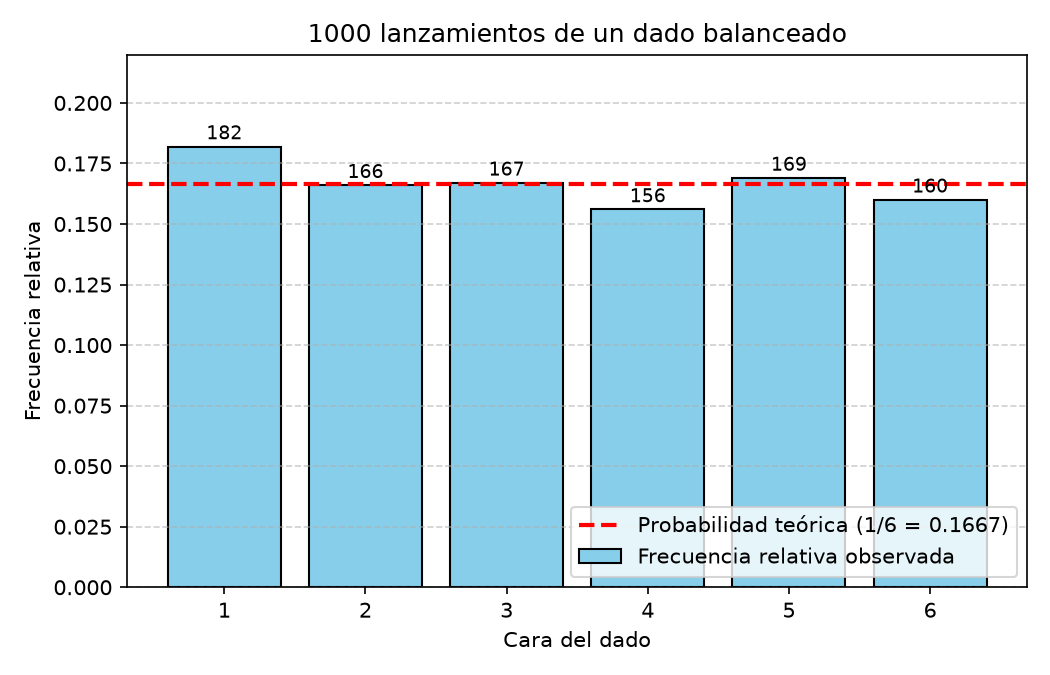
\includegraphics[width=0.75\textwidth]{img/a_dado_barras.png}
\caption{Frecuencia relativa de cada cara en 1000 lanzamientos de un dado balanceado. Los números sobre las barras son las frecuencias absolutas y la línea roja, la probabilidad teórica $1/6$.}
\label{fig:dado}
\end{figure}

\begin{itemize}
    \item \textbf{Frecuencias relativas.} Las seis frecuencias relativas están entre 0.156 y 0.182, muy cerca de la probabilidad teórica de $1/6 \approx 0.1667$, y suman exactamente 1. La cara 1 es la que más se aleja, con 182 apariciones (0.0153 por encima de $1/6$), y la cara 4 la que menos salió, con 156. Las caras 2, 3 y 5 quedaron a menos de 0.003 de la probabilidad teórica.
    \item \textbf{¿Son diferencias reales?} En la Figura~\ref{fig:dado} las barras no son exactamente iguales, pero la prueba chi-cuadrada da $p = 0.792$, muy por encima de 0.05. Las diferencias observadas son las que se esperan por azar en 1000 lanzamientos, y no hay evidencia de que el dado esté cargado.
    \item \textbf{Media y varianza.} La media de los lanzamientos (3.444) y su varianza (2.972) están muy cerca de los valores teóricos $E[X] = 3.5$ y $\operatorname{Var}[X] = 2.917$. Esto confirma que la muestra reproduce no solo las probabilidades de cada cara, sino también el centro y la dispersión de la distribución.
\end{itemize}

\subsection{Tarea b: Muestras de la distribución normal}

\begin{consola}[label=out:b]{Ejecución de \texttt{act07.py}: Tarea b}
=== b) Variable continua: 500 muestras de N(100, 15) ===
                Poblacional  Muestral  Diferencia  Error relativo (%)
Media                   100    99.026      -0.974              -0.974
Desv. estándar           15    14.666      -0.334              -2.228

Error estándar de la media (sigma / raíz de n): 0.671
Diferencia de la media en errores estándar: -1.45
Mínimo: 53.76   Máximo: 142.92

Proporción de muestras en cada intervalo:
           Muestra (%)  Teórica (%)
[85, 115]         70.0         68.3
[70, 130]         96.2         95.4
[55, 145]         99.8         99.7
\end{consola}

\begin{figure}[htbp]
\centering
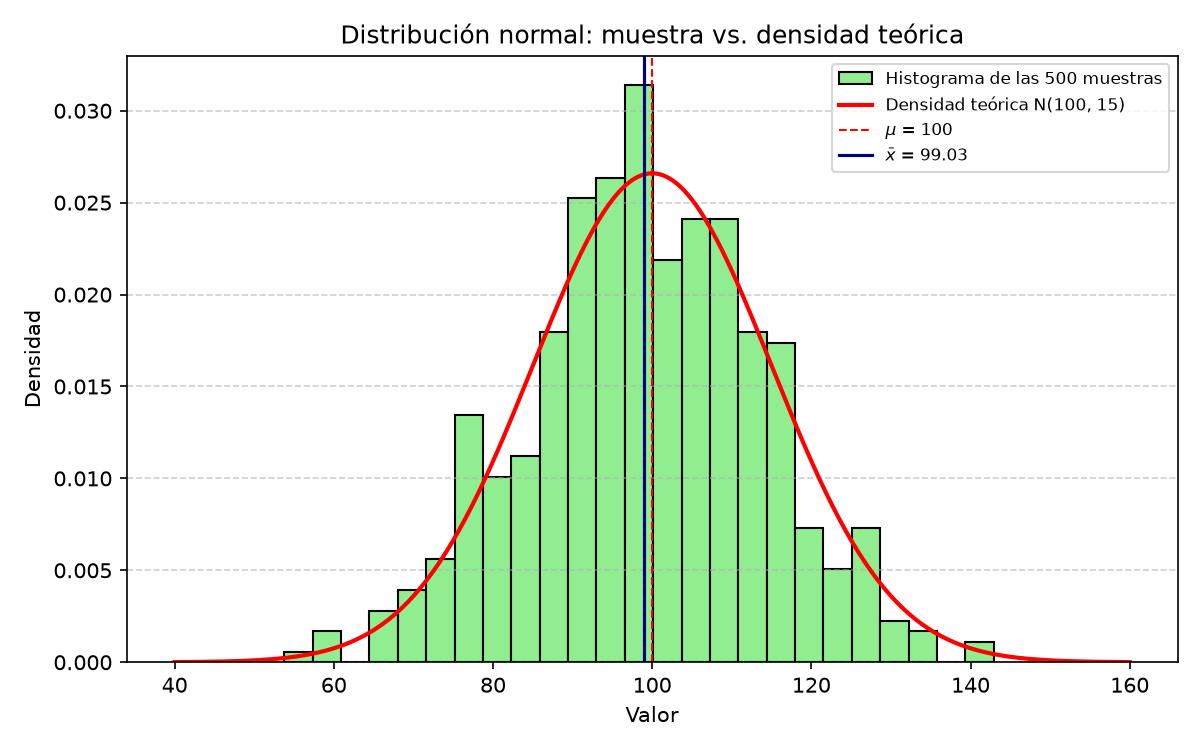
\includegraphics[width=0.78\textwidth]{img/b_normal_histograma.png}
\caption{Histograma de densidad de 500 muestras de una distribución normal con $\mu = 100$ y $\sigma = 15$, con la densidad teórica superpuesta.}
\label{fig:normal}
\end{figure}

\begin{itemize}
    \item \textbf{Forma.} El histograma de la Figura~\ref{fig:normal} sigue la forma de campana de la densidad teórica: es simétrico, con el máximo cerca de 100, y las frecuencias decrecen hacia ambos lados. Algunas barras quedan por encima o por debajo de la curva, como la de 95 a 100, que es la variación natural de una muestra finita.
    \item \textbf{Media.} La media muestral es 99.026, a menos de un punto de $\mu = 100$ (un error relativo de $-0.97$\,\%). El error estándar de la media es $15/\sqrt{500} = 0.671$, por lo que la diferencia equivale a 1.45 errores estándar: está dentro del rango de $\pm 2$ errores estándar que se espera por azar.
    \item \textbf{Desviación estándar.} La desviación estándar muestral es 14.666, un 2.2\,\% menor que $\sigma = 15$.
    \item \textbf{Proporciones.} El 70.0\,\%, el 96.2\,\% y el 99.8\,\% de las muestras quedaron a una, dos y tres desviaciones estándar de la media, cerca del 68.3\,\%, 95.4\,\% y 99.7\,\% que predice la distribución normal. Los valores van de 53.76 a 142.92, es decir, ninguno se aleja más de tres desviaciones estándar de la media.
\end{itemize}

Los estadísticos muestrales no coinciden exactamente con los parámetros poblacionales porque se calcularon a partir de una sola muestra de 500 valores. Otra muestra daría valores ligeramente distintos, pero, como muestra la siguiente sección, todos ellos se acercan a $\mu$ y $\sigma$ al aumentar el tamaño de la muestra.

\subsection{Extensión: convergencia}

\begin{consola}[label=out:ext]{Ejecución de \texttt{act07.py}: convergencia}
=== Extensión: convergencia ===
Dado, n =   10: máxima |frecuencia relativa - 1/6| = 0.1667
Dado, n =  100: máxima |frecuencia relativa - 1/6| = 0.0933
Dado, n = 1000: máxima |frecuencia relativa - 1/6| = 0.0153
Normal, n =  10: media acumulada = 101.11
Normal, n = 100: media acumulada = 100.18
Normal, n = 500: media acumulada = 99.03
\end{consola}

\begin{figure}[htbp]
\centering
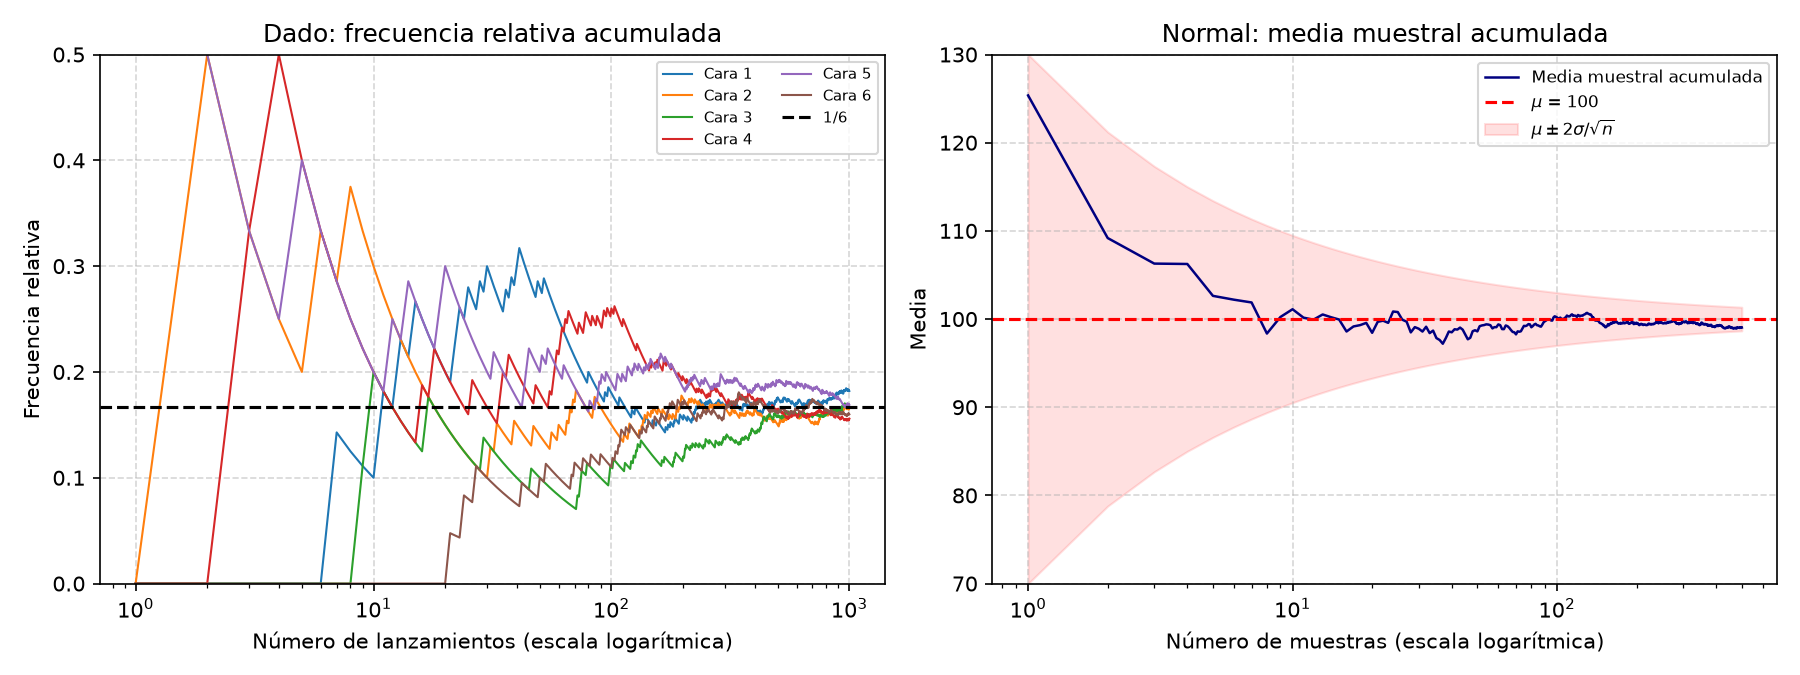
\includegraphics[width=\textwidth]{img/convergencia.png}
\caption{Izquierda: frecuencia relativa acumulada de cada cara del dado. Derecha: media acumulada de las muestras normales, con la banda $\mu \pm 2\sigma/\sqrt{n}$. En ambos casos el eje horizontal está en escala logarítmica.}
\label{fig:convergencia}
\end{figure}

La Figura~\ref{fig:convergencia} muestra que, con pocas observaciones, los estimadores son muy inestables: después de 10 lanzamientos alguna cara todavía no había salido, por lo que su frecuencia relativa se alejaba $1/6$ de la probabilidad teórica, y la media de las primeras muestras normales llegó a superar 120. Al aumentar las observaciones, las seis frecuencias relativas se concentran alrededor de $1/6$ (la máxima desviación baja de 0.167 con 10 lanzamientos a 0.093 con 100 y a 0.015 con 1000), y la media acumulada se estabiliza cerca de 100, dentro de la banda $\mu \pm 2\sigma/\sqrt{n}$, que se estrecha conforme crece $n$. Este es el comportamiento que describe la teoría: con más mediciones, la distribución muestral se aproxima a la distribución teórica \parencite{bonamente2017}.

\subsection{Tarea c: Análisis comparativo}

\begin{consola}[label=out:c]{Ejecución de \texttt{act07.py}: Tarea c}
=== c) Clasificación de variables en conjuntos de datos reales ===
                       Conjunto     dtype  Valores distintos                   Tipo
outlook                 Weather       str                  3  Discreta (categórica)
temperature             Weather       str                  3  Discreta (categórica)
humidity                Weather       str                  2  Discreta (categórica)
windy                   Weather      bool                  2  Discreta (categórica)
play                    Weather       str                  2  Discreta (categórica)
temperature        Weather num.   float64                 12               Continua
humidity           Weather num.   float64                 10               Continua
sepal length (cm)          Iris   float64                 35               Continua
sepal width (cm)           Iris   float64                 23               Continua
petal length (cm)          Iris   float64                 43               Continua
petal width (cm)           Iris   float64                 22               Continua
species                    Iris  category                  3  Discreta (categórica)

Resolución de medición de las variables continuas:
  Weather temperature (°F)   rango [64, 85], diferencia mínima entre valores: 1.0
  Weather humidity (%)       rango [65, 96], diferencia mínima entre valores: 1.0
  Iris sepal length (cm)     rango [4.3, 7.9], diferencia mínima entre valores: 0.1

Figuras guardadas en img/
\end{consola}

La Tabla~\ref{tab:comparativa} resume las diferencias entre ambos tipos de variables aleatorias a partir del marco conceptual y de las simulaciones realizadas.

\begin{table}[htbp]
\centering
\caption{Comparación entre variables aleatorias discretas y continuas.}
\label{tab:comparativa}
\small
\begin{tabular}{>{\bfseries\raggedright\arraybackslash}p{2.9cm}>{\raggedright\arraybackslash}p{5.9cm}>{\raggedright\arraybackslash}p{5.9cm}}
\hline
\textbf{Característica} & \textbf{Variable discreta} & \textbf{Variable continua} \\
\hline
Valores posibles & Conjunto finito o numerable de estados & Cualquier valor real dentro de un rango \\
Cómo se obtiene & Se cuenta o se clasifica & Se mide \\
Función que la describe & Función de masa de probabilidad, $P(X = x)$ & Función de densidad, $f(x)$ \\
Probabilidad de un valor exacto & Puede ser mayor que cero, por ejemplo $P(X = 3) = 1/6$ & Es cero; solo los intervalos tienen probabilidad \\
Cálculo de probabilidades & Suma de probabilidades & Área bajo la curva (integral) \\
Gráfico adecuado & Diagrama de barras & Histograma y curva de densidad \\
Distribuciones típicas & Uniforme discreta, Bernoulli, binomial, Poisson & Normal, exponencial, gamma \\
Ejemplo simulado & Cara de un dado: $\{1, \ldots, 6\}$, $E[X] = 3.5$ & $N(100, 15)$: valores reales, de 53.76 a 142.92 en la muestra \\
Ejemplos en Weather & \texttt{outlook}, \texttt{windy}, \texttt{play} y la versión nominal de \texttt{temperature} y \texttt{humidity} & \texttt{temperature} (°F) y \texttt{humidity} (\%) en la versión numérica \\
Ejemplos en Iris & \texttt{species} (setosa, versicolor, virginica) & Longitud y ancho del sépalo y del pétalo (cm) \\
Tipo en \texttt{pandas} & \texttt{str} (\texttt{object} antes de pandas 3), \texttt{category}, \texttt{bool} o entero & \texttt{float64} \\
\hline
\end{tabular}
\end{table}

A partir de la clasificación de la Salida~\ref{out:c} se observa lo siguiente:

\begin{itemize}
    \item \textbf{Weather Dataset nominal.} Las cinco variables son discretas categóricas: \texttt{outlook} toma 3 estados (sunny, overcast, rainy), \texttt{windy} es booleana y la clase \texttt{play} tiene 2 valores. En esta versión, incluso la temperatura y la humedad son discretas, porque se registraron como categorías (hot, mild, cool; high, normal).
    \item \textbf{Weather Dataset numérico.} La misma temperatura y humedad son variables continuas cuando se registran como medidas: la temperatura va de 64 a 85\,°F y la humedad de 65 a 96\,\%. Esto muestra que el tipo de una variable depende también de cómo se mide y se registra el fenómeno.
    \item \textbf{Iris Dataset.} Las cuatro medidas de las flores son continuas y la especie es discreta. La longitud del sépalo, por ejemplo, toma 35 valores distintos en 150 flores, mientras que la especie solo toma 3.
    \item \textbf{Resolución de medición.} Las variables continuas se registran con una precisión finita: la temperatura y la humedad del Weather Dataset en unidades enteras, y las medidas de Iris en décimas de centímetro. Por eso en la práctica toman un número limitado de valores distintos, aunque conceptualmente puedan tomar cualquier valor dentro de su rango.
\end{itemize}

\begin{figure}[htbp]
\centering
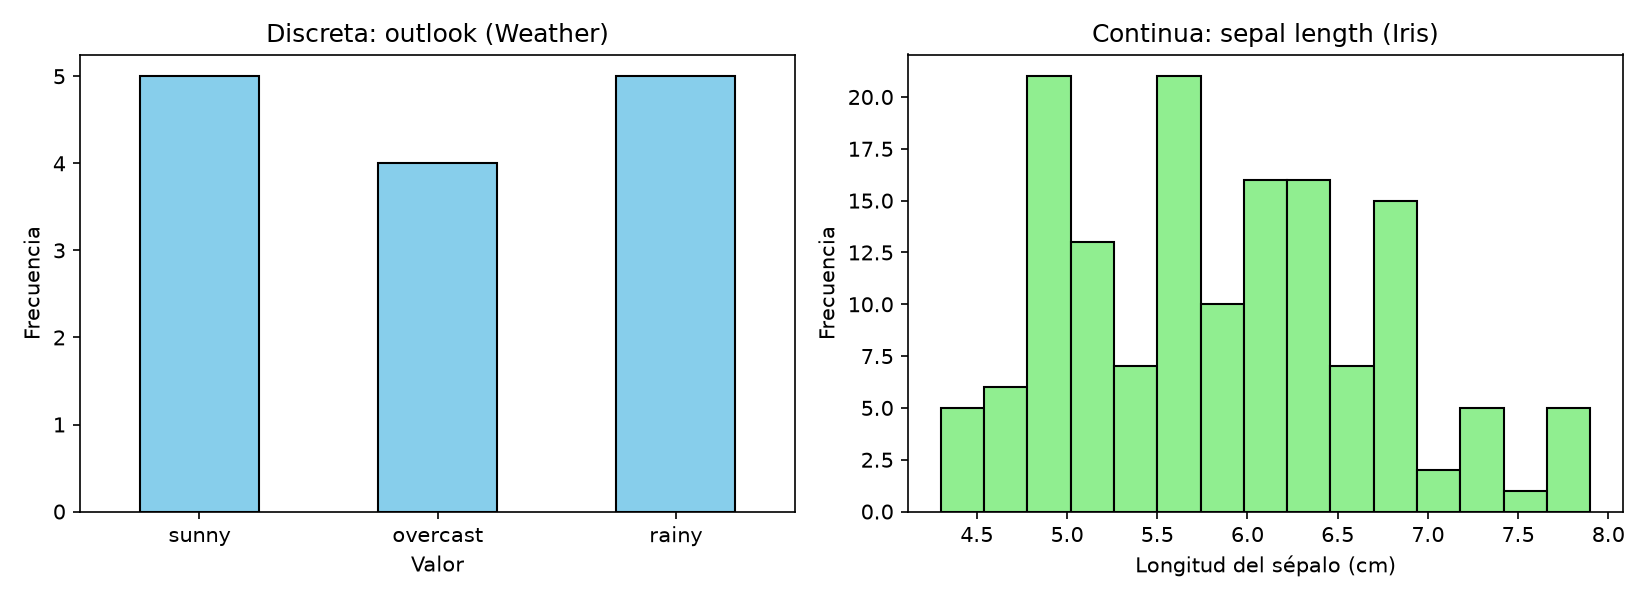
\includegraphics[width=0.9\textwidth]{img/c_discreta_continua.png}
\caption{Izquierda: diagrama de barras de una variable discreta (\texttt{outlook} del Weather Dataset). Derecha: histograma de una variable continua (longitud del sépalo del Iris Dataset).}
\label{fig:comparacion}
\end{figure}

La Figura~\ref{fig:comparacion} muestra la diferencia en la forma de representarlas: una variable discreta se resume con una barra por cada estado posible, mientras que una variable continua necesita agruparse en intervalos para construir un histograma.

\section{Conclusiones}

Las simulaciones permitieron observar de forma directa la diferencia entre variables aleatorias discretas y continuas. El dado toma solo seis valores, cada uno con una probabilidad positiva de $1/6$, y su distribución se representa naturalmente con un diagrama de barras. La variable normal, en cambio, toma valores reales que casi nunca se repiten, por lo que su distribución solo puede describirse con una densidad y representarse agrupando los valores en un histograma.

En ambos casos, la muestra reprodujo la distribución teórica con diferencias pequeñas: las frecuencias relativas del dado se alejaron como máximo 0.015 de $1/6$, y la media y la desviación estándar de la muestra normal quedaron a menos del 2.5\,\% de $\mu$ y $\sigma$. Las extensiones permitieron ir más allá de la comparación visual: la prueba chi-cuadrada confirmó que las diferencias del dado son compatibles con el azar, el error estándar mostró que la diferencia entre $\bar{x}$ y $\mu$ es la esperada para 500 muestras, y las gráficas de convergencia mostraron cómo los estimadores se estabilizan al aumentar el número de observaciones.

Finalmente, el análisis de los conjuntos Weather e Iris mostró que en los datos reales conviven ambos tipos de variables y que el tipo depende de cómo se registra el fenómeno: la temperatura es discreta en la versión nominal del Weather Dataset y continua en la numérica. Identificar correctamente el tipo de cada variable es un paso previo indispensable para elegir la distribución, el gráfico y el modelo adecuados, por ejemplo, en un clasificador Naive Bayes que trata de forma distinta las características categóricas y las numéricas.

\referencias

\end{document}
